\documentclass[a4paper, 11pt]{article}

\usepackage{natbib}
\bibliographystyle{agsm}
\setcitestyle{authoryear,open={(},close={)}}

\usepackage{fontspec}
\setmainfont[Ligatures=TeX]{Lato Light}

\usepackage{graphicx}
\usepackage{wrapfig}

\linespread{1.05}

\makeatletter
\renewcommand{\maketitle}{
\begin{flushright}
{\LARGE\@title}

\vspace{50pt}

{\large\@author}
\\\@date 
\vspace{40pt}
\end{flushright}
}
\renewcommand{\@seccntformat}[1]{}
\makeatother


\title{\textbf{Essay}\\Sub title on Essay}

\author{\textsc{Ans Vaessen}
\\{\textit{ans@nlgids.london}}}

\date{\today}

%%%%%%%%%%%%%%%%% START %%%%%%%%%%%%%%%%%%

\begin{document}
\maketitle

\begin{abstract}
This is an abstract.
\end{abstract}

\vspace{30pt} % Some vertical space between the abstract and first section

\section*{Introduction}
Is Ryanair an disruptive entrant in the flight industry?


Flying used to be an expensive mode of travel until the low cost airlines entered the market. In 1995 two airlines came with a new concept: Low Cost Airlines. This was an innovation that changed the airline business as we know it. \cite{TiddBessant} use it as an example to explain disruptive innovation. \citep{Christensen97} explains his model for disruptive innovation in the innovator's dilemma. The elements is model for disruptive innovation are used to explain if the ryanair is a good example of a disruptive entrant in the airline business.


See \cite{Christensen97}.
See \citep{Christensen97}.
See \citep[p. 145]{Christensen97}.

\section{Ryanair and change of regulations}

In 1984 Ryanair was founded and in the beginning of the nineties started with low cost flights by copying the 'no frills' model from Southwest airlines in the United States of America. Calling themself Europe’s first low fares airline \cite{Ryanair}. 'No frills' meant, no meals, no seat allocation and also moving to a single aircraft type and using small underused airports while offering the lowest fares \citep{Diaconu}.

Helped by the new European Union deregulation, to promote international trade, Ryanair could expand and increase their flights in this liberalized aviation market \citep{Diaconu}. \cite{TiddBessant} describe regulation as a source of innovation that works as a two sided sword, restricting on one side and deregulation, as in this example, can create new opportunities for innovation.

Flights used to be regulated by countries, each country had their own national airline. British Airways (BA) for Britain and
Royal Dutch Airlines (KLM) for the Netherlands. Governments would agree between nations on flying schedules, amount of
passengers and fares. There was no competition until the European Commission introduced a reform process that changed the
rules. "Since April 1997, any airline holding a valid Air Operators Certificate in the EU can operate on any route within the
European Union, including wholly within another country, without restriction on price or capacity. As a result, European air
travel has been flooded with an influx of low-cost airlines \citep{Eurocontrol2017}.


\label{sec:this-is-a-section}

\section{The Innovator's Dilemma}


In his book \cite{Christensen97} describes the innovator's dilemma and how incumbent fail. He describes how big companies sustain their growth by improving their products and performances. Often in an incremental way, little steps at the time to fine tune and do better what they do good, it can be in a radical ways as well. In \citep{Christensen97} explains how the hard disk drive industry got disrupted multiple times. Could this also be the case for national airlines like BA and KLM are they disrupted by the so called low cost carriers like Ryanair?

According to Christensen \cite{Christensen97} there are 3 elements causing disruption: Firstly, big companies want to better their performance. This can be done by innovation but has as goal to make a better product for the customer. Disruptive technology happens when new entrants enter the market. The entrants start at the fringe, or low-end market to sell an inferior product, often cheaper or simpler, or both, than the original product. These entrants target a niche-market with less demanding customers. Secondly, the incumbents in their attempt to improve the product overshoot the mainstream market, whereas the new entrants have been improving their cheaper and simpler product and move into the mainstream market.Finally as a third element \cite{Christensen97} points out that the main industry can't react to the disruption because the entrants target a small market with low margins. This is of no interest to the big companies. They need to grow and make more profit, for that they need higher margins. Furthermore, their customers demand a high quality product, they do not want a simpler product, and often inferior product.

Figure \ref{fig:graph1} illustrates how this works. The big company is sustaining the technology and performs better over time. So much so that they leave the mainstream and end up in the high end market. At the same time the new entrant is improving its product and enters the mainstream in time to take over from the incumbent \cite{Christensen97}.

\begin{figure}[h!]
    \centering
    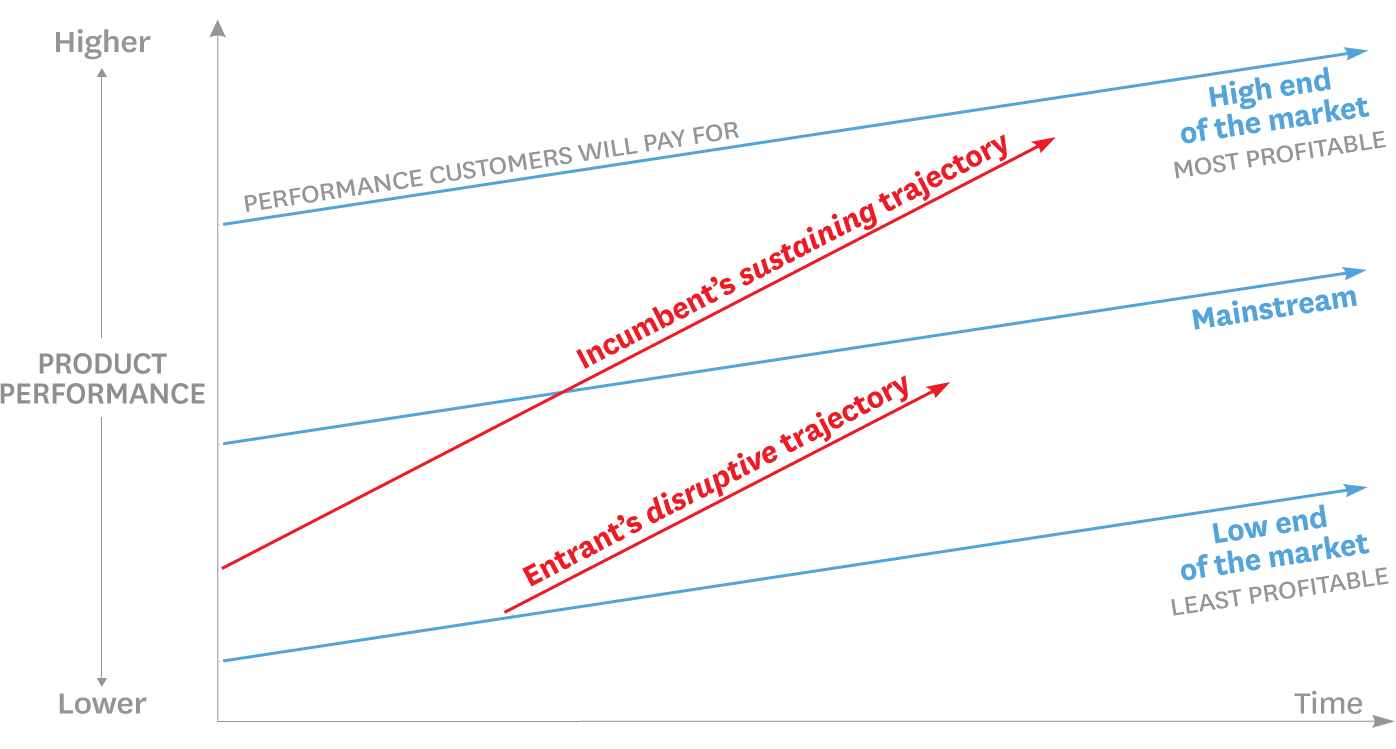
\includegraphics[width=0.9\textwidth]{big-model.png}
    \caption{The figure from \cite{Christensen2015}.}
    \label{fig:graph1}
\end{figure}

The rise of the low cost carriers like Ryanair is often called an disruptive innovation.
But how do these elements hold up when applied to the airline business and in this case Ryanair in particular.


\subsection{Ryanair as an Entrant}


The Incumbents in this case are national airlines like BA and KLM. On their flights they provided food and unlimited drinks, allocated seats, generous baggage allowance and overall good service. Flights leave from prime location and main easy to reach airports. Flights leave on prime times for a high price. They want to better their performance. \cite{Christensen97} than continuous to describe how this can be disrupted by newcomers that offer a product of worse quality than the incumbent. Although in in the beginning not seen as a threat because of the inferior design or performance it can sometimes turn out to be the cause of big firms failure.

Looking at Ryanair's product, \cite{Barrett} notes that Ryanair dropped customer service items compared to the National European Airlines. No extra's on the flight and more seats per aircraft. Another major difference is the airport service, by using secondary airports like London Luton instead of Heatrow, these airports charge lower landing charges. A third observation by \cite{Barrett} is the fact that tickets are sold directly to the customer not via a travel agent this is cutting the cost. Kenny Jacobs, Chief Marketing Officer, Ryanair says: "On their first flight customers paid in cash, which was collected in a bucket as customers departed" \citep{ITBberlin}.

An other point is low maintenance because use of a single air craft (needs citation)

Instead of entering the regular market the Low Cost Airlines looked for new markets at the fringe. This is consistent with
\cite{Christensen2015} first element.


The main airlines kept doing what they do best and maybe even overshoot the mainstream market by adding more and more 'frills'. \cite{Droege} describes it as value-added attributes, like food and drinks that become standard for mainstream customers. But more new users enter the market and start flying with low cost carries like Ryanair. Their market-share grew, and these new travellers talked about this 'good enough' flight and the regular existing market including business travellers heard about it and took an interest in these 'cheaper' but good enough flights, especially on short haul flights \citep{TiddBessant}.

Fare reduction was the first step to enter a new fringe market but they attracted other regular customers as well and not only because of the 'good enough' flights. Additionally, there was also improvements in the service that attracted people. According to \cite{Barrett} Ryanair looses less bags and they excel in punctuality when it comes to arrival times, on these service levels they score better than national carriers like BA or Air Francein 2004. He \citep{Barrett} than continues to explain that this is due to the fact that Ryanair offers a simple product, no connecting flights and uses smaller airports, which makes it easier to meet these levels of service. Furthermore the secondary airports have other appeals like shorter walking distance and less congestion at the border control and check in.

As explained by \cite{Christensen2015} the next step would be that the incumbent overshoots the target and the entrants move into
the mainstream market. It is interesting to see this might have been the case at the start of the millenium but quickly the
incumbent reacted. Still providing leg space and free food and drinks for the demanding customer in Business and sometimes
First Class. The Economy travel can travel cheaper and get's less "frills'. In his article "End of the free lunch?"
\cite{Dennis} argues that the European National airlines adopted many of the low cost mechanisms of the low cost carriers. For
example BA started operating point-to-point routes and making use of regional airports to do so. Cheaper fares with more
conditions and flexible fares for a higher price. At the time when \cite{Dennis} wrote this article lunches were still free
however, since the beginning of 2017 BA out sourced the catering to Marks \& Spencer \citep{Calder}.


\subsection{Ryanair Moving into Mainstream?}
\label{limits}


Low Cost Carriers (LCC) managed to increased their market share as this Figure \ref{fig:graph2} illustrates. So even though the traditional airlines reacted as described by \citep{Dennis} the LCC share of total flights grew from 19 percent in 2007 to 30 percent in 2016, whereas the traditional carriers, market segment decreased between 2007 and 2016. Within this LLC share Ryanair is responsible for the biggest part with 22 percent \citep{Eurocontrol2017}

\begin{figure}[h!]
    \centering
    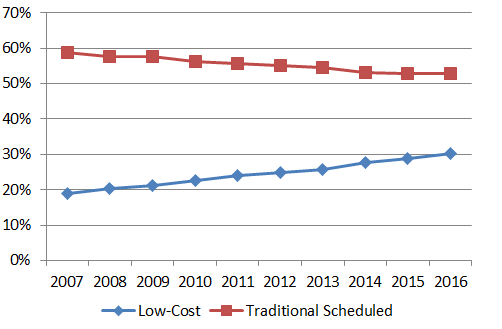
\includegraphics[width=0.9\textwidth]{evolution-lcc-vs-tradsched.png}
    \caption{The figure from \cite{Eurocontrol2017}.}
    \label{fig:graph2}
\end{figure}

\citep{Christensen2015} uses the case of UBER to further explain how to apply the model for disruptive innovation correctly. "Uber has quite arguably been increasing the total demand - that's what happens when you develop a better, less-expensive solution to a widespread customer need"\citep[p. 4]{Christensen2015}. He than continues that disrupters are not mainstream until increase their quality. Looking at Ryan air it is fair to say that they did increase their share of flights but the total amount of flights increased as well \citep{Eurocontrol2018} but have not improved their quality or have been sustaining their innovation into mainstream. The opposite seems true as \citep{Barrett} writes the demand for cheap flights like Ryanair will probably remain high as long as the fare price is low and Ryanair stays on the trajectory of cutting cost and not engage in expensive projects like new logo's and fancy headquarters. \cite{Eurocontrol2018} identifies low cost carriers have helped traffic grow and also that some are trying to penetrate the longhaul market. To offer these longhaul flights for a cheaper fare is harder to achieve because of operating Longhaul flights is more expensive when it comes to aircraft, fuel and crew. They loose the cost effective advantage.


\subsection{Incumbent Can Not React}
\label{reaction}

Lastly to fit all the elements of the disruptive innovation \cite{Christensen97} claims incumbents can't react because of their existing customers and shareholders who do not allow them to offer an inferior product.
Be that as it may an anonymous expert in \cite{King} explains the barrier to react in the case of the airline industry is a structural barrier. For competing with a low-cost-carrier on the same businessmodel, the airline would need new aircrafts, workers, airports, gates etcetera and the best response is not to adapt.

As explained before adapting is what the main airlines eventually did by copying what worked for the traditional airlines. like online booking and check in and less 'frills' for the less demanding price conscious customers. At the same time they kept on focussed on their high end market. Furthermore a  Sometimes still focus on the main market their is still a big profit to be made \cite{Christensen2015}.


\section{Conclusion}

Although the rise of Ryanair has elements of disruptive innovation it doesn't fit the model completely. Ryanair as a low cost carrier is a new entrant in airline business. They started at the fringe and are grew their marketshare, expanded and took passengers from the mainstream on board. The incumbent like BA have overshoot their customer needs especially on shorthaul flights they moved to the cheaper flights.

Ryanair however has, instead of sustaining their product and adding quality to really move into mainstream, set their goal to keep costs low and charging people for extra's. In other words they are staying in the lower end of the mainstream. The incumbent on the other side adapted the new, low cost, business model where possible. While at the same time keeping their more demanding and more profit making customers.

\cite{Christensen2015} explains there are a couple of points that are overlooked in using the model of disruptive innovation. He states it is a process and incumbents can be creative in the defense and that incumbent do not need to respond but should continue to provide for their core customers.

The incumbents did not flounder and at this moment the two models stand next

The future will tell if the two business models will survive next to each other or not.

\cite{Diaconu}, recommends Ryanair to start flying from the mainairports to get hold of the business travellers more and like \cite{Eurocontrol2018} describes there is an attempt to penetrate the longhaul market. When Ryanair succeeds in these and other changes they would fit the model better. But as \cite{Christensen2015} warns the main airlines might be creative and out smart the Low cost Carriers like Ryanair.

\ldots




%% disable some things
\renewcommand{\textbf}{}
\renewcommand{\bf}{}
\bibliography{biblio}{}
\end{document}
